\documentclass{article}
\usepackage{tikz}
\usetikzlibrary{matrix}

\begin{document}

\begin{figure}[h]
    \centering
    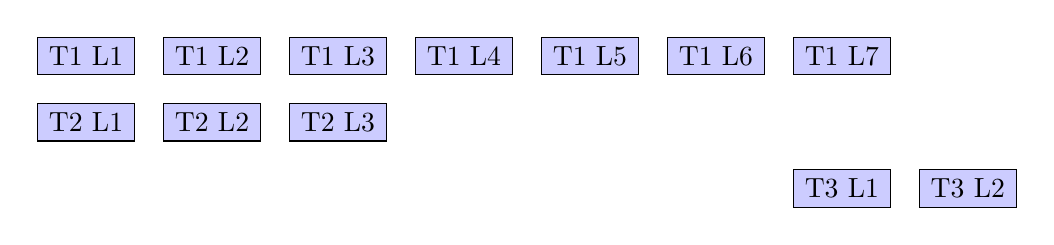
\begin{tikzpicture}
        \matrix (m) [matrix of nodes, row sep=1em, column sep=1em, nodes={draw, fill=blue!20, text width=1cm, align=center}]
        {
            T1 L1 & T1 L2 & T1 L3 & T1 L4 & T1 L5 & T1 L6 & T1 L7 \\
            T2 L1 & T2 L2 & T2 L3 &       &       &       &       \\
            &       &       &       &       &       & T3 L1 & T3 L2 \\
        };
    \end{tikzpicture}
    \caption{The different levels of the data challenge. There are 7 filtering levels, 3 reverb levels and 2 combined levels. The specifics of the levels are explained in Table \ref{tab:exp}.}
    \label{fig:levels}
\end{figure}

\end{document}